\documentclass[11pt]{article}
\usepackage[utf8]{inputenc}
\usepackage[T1]{fontenc}
\usepackage{graphicx}
\usepackage{grffile}
\usepackage{longtable}
\usepackage{wrapfig}
\usepackage{rotating}
\usepackage[normalem]{ulem}
\usepackage{amsmath}
\usepackage{textcomp}
\usepackage{amssymb}
\usepackage{capt-of}
\usepackage{hyperref}
\usepackage{minted}
\author{Student: Brian Cheung bc32427 \\ Professor: Mohit Tiwari \\ TA: Antonio Espinoza \\ Department of Electrical \& Computer Engineering \\ The University of Texas at Austin}
\date{\today}
\title{EE379K Enterprise Network Security Lab 1 Report}
\hypersetup{
 pdfauthor={Student: Brian Cheung bc32427 \\ Professor: Mohit Tiwari \\ TA: Antonio Espinoza \\ Department of Electrical \& Computer Engineering \\ The University of Texas at Austin},
 pdftitle={EE379K Enterprise Network Security Lab 1 Report},
 pdfkeywords={},
 pdfsubject={},
 pdfcreator={},
 pdflang={English}}
\begin{document}

\maketitle
\section{Part 1 - Server and Client Networking}
\label{sec:part-1}
The task was to implement an echo server and client in C given a Python implementation that modeled the desired behavior of the server and client.
The Python implementation was also used to test the compatibility of the C program by interchanging the server and client with a Python server and C client and vice versa.
The next task was to perform a Denial of Service (DOS) attack on the C server.
\subsection{Step 1 - Echo Server}
\subsubsection{Build server and client}
In a terminal window, start at root directory of project and run the following commands:
\begin{minted}{bash}
  $ cd Part\ 1
  $ make
\end{minted}
\subsubsection{Run server and client}
Run the following commands to start the server:
\begin{minted}{bash}
  $ cd Part\ 1
  $ ./server
\end{minted}
Open a new terminal window and run the following commands to start the client:
\begin{minted}{bash}
  $ cd Part\ 1
  $ ./client
\end{minted}
\subsection{Step 2 - DOS Attack}
The DOS attack was performed using a program called \textbf{\emph{hping3}}.
The attacker flooded the server with SYN packets while using a spoofed IP address to hide the source IP address.
Without the correct IP, the server was unable to send SYN and ACK packets back to the attacker,
which prevented the three-way handshake from being completed.
This prevents the server from processing other clients' requests because it is too busy trying to complete the attacker's requests,
so clients that want to connect to the server are left waiting.

The following command was used to perform the DOS attack:
\begin{minted}{bash}
  $ sudo hping3 -S -w 64 -p 12000 --flood --rand-source 127.0.0.2
\end{minted}
\textbf{\emph{hping3}} command flags and options:

\textbf{-S}: flood with SYN packets

\textbf{-p}: 12000: port 12000

\textbf{--flood}: send packets as fast as possible

\textbf{--rand-source}: generates a spoofed IP address to hide the source IP

\textbf{127.0.0.2}: IP address of server
\newline

The recorded pcap of the attack, shown in Figure \ref{fig:pcap-screenshot}, displays the flood of SYN packets sent to the server.
Furthermore, the source IP of the attacker is randomly generated each time and there are no ACK packets, which prevents the handshake from being completed.
\begin{figure}[htbp]
\centering
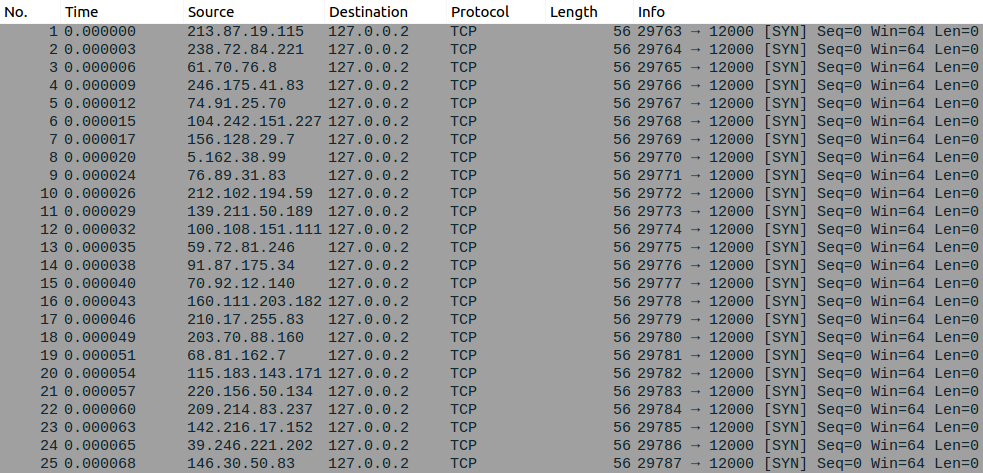
\includegraphics[width=.9\linewidth]{./pcap-screenshot.png}
\caption{\label{fig:pcap-screenshot}
A screenshot of the pcap in Wireshark during a DOS attack.}
\end{figure}

\section{Part 2 - Scan the Internet}
\label{sec:part-2}

Total number of machines probed: 16063066
Number of machines that responded: 11448
Hitrate: 0.071\%

\section{Part 3}

\label{sec:part-3}
part 3 paragraph

\begin{minted}{c++}
  int main() {
    printf("Hello World");
    return 0;
  }
\end{minted}

\section{Part 4}
\label{sec:part-4}

\section{Conclusion}
\label{sec:conclusion}
Please provide feedback so we can improve the labs for the course. How many
hours did the lab take you? Was this lab boring? Did you learn anything? Is
there anything you would change? Feel free to put anything here, but leaving it
blank will result in the loss of points.

\bibliography{bibliography}
\bibliographystyle{ieeetr}
\end{document}
